\documentclass[tikz,border=10pt]{standalone}
\usepackage{amsmath}

\tikzset{
    block/.style={rectangle, draw, fill=blue!20, text width=5em, text centered, rounded corners, minimum height=4em},
    line/.style={draw, -stealth, thick},
}

\begin{document}
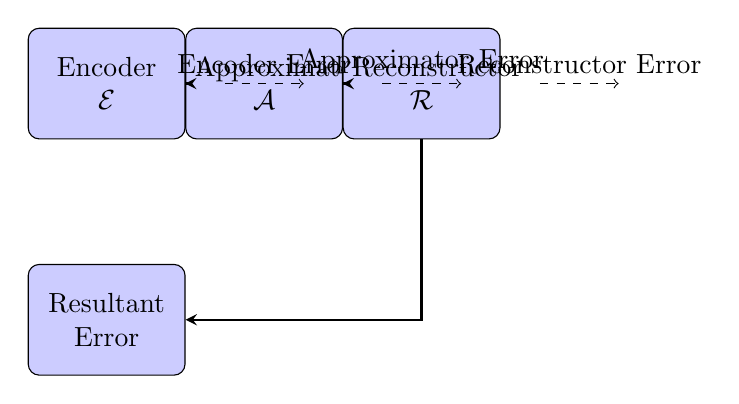
\begin{tikzpicture}[node distance=2cm]

\node[block] (Encoder) {Encoder \\ \(\mathcal{E}\)};
\node[block, right of=Encoder] (Approximator) {Approximator \\ \(\mathcal{A}\)};
\node[block, right of=Approximator] (Reconstructor) {Reconstructor \\ \(\mathcal{R}\)};
\node[block, below of=Encoder, node distance=3cm] (Error) {Resultant Error};

% Draw lines between blocks
\draw[line] (Encoder) -- (Approximator);
\draw[line] (Approximator) -- (Reconstructor);
\draw[line] (Reconstructor) |- (Error);

% Draw arrows to show error components
\draw[->, dashed] (Encoder.east) ++(0.5,0) -- ++(1,0) node[midway, above] {Encoder Error};
\draw[->, dashed] (Approximator.east) ++(0.5,0) -- ++(1,0) node[midway, above] {Approximator Error};
\draw[->, dashed] (Reconstructor.east) ++(0.5,0) -- ++(1,0) node[midway, above] {Reconstructor Error};

\end{tikzpicture}
\end{document}